% Source for the figure of the table of the 0-1 knapsack (sec. 13.7): the
% instance p = (3,2,4,2), v = (2,1,3,2), C = 5, and the cells read back.
% Build: make figures (in ../build).
\documentclass[border=4pt]{standalone}
\usepackage[T1]{fontenc}
\usepackage{newpxtext,newpxmath}
\usepackage[varqu,varl,scaled=0.95]{zi4}
\usepackage{tikz}
% tikz-ads.tex: the TikZ styles shared by the figures of the memory of the
% manual, \input by each standalone figure: a cell of a vector (cell), the
% cell that an operation touches (touched), a free cell (free), a node of a
% linked structure (node), the labels of indices (index) and of variables
% (var), a pointer (ptr), and \cells and \indices to draw a row of cells.
\usetikzlibrary{arrows.meta,positioning,calc,fit,shapes.multipart}
\definecolor{adsTouched}{RGB}{214,196,236}
\definecolor{adsFree}{RGB}{236,236,236}
\tikzset{
  ads/.style={>={Stealth[length=2mm]},font=\small,
              every node/.append style={inner sep=0pt}},
  cell/.style={draw,minimum width=7mm,minimum height=7mm,
               font=\small\ttfamily,outer sep=0pt},
  touched/.style={cell,fill=adsTouched},
  free/.style={cell,fill=adsFree,text=black!45},
  node/.style={draw,rounded corners=1pt,minimum width=8mm,
               minimum height=6mm,font=\small\ttfamily},
  index/.style={font=\scriptsize\ttfamily,text=black!60},
  var/.style={font=\small\itshape},
  ptr/.style={->,thick}
}
% \cells{name}{x,y}{list}: a row of cells, the first at (x,y), named
% name-0, name-1, ...; each item is text/style, the style one of cell,
% touched and free (e.g., {a/cell,e/touched,/free})
\newcommand{\cells}[3]{%
  \foreach \v/\s [count=\i from 0] in {#3}
    \node[\s] (#1-\i) at ($(#2)+(\i*7mm,0)$) {\v};}
% \indices{name}{n}: the indices 0 .. n-1 under the cells of name
\newcommand{\indices}[2]{%
  \foreach \i in {0,...,\numexpr#2-1\relax}
    \node[index,below=1.2mm of #1-\i] {\i};}

\begin{document}
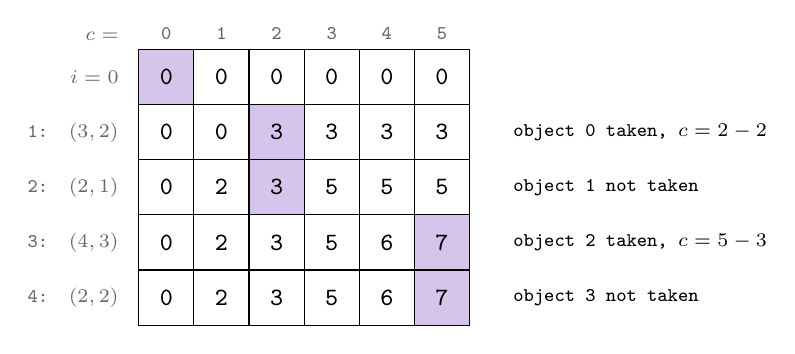
\begin{tikzpicture}[ads]
  \cells{r0}{0,0}{0/touched,0/cell,0/cell,0/cell,0/cell,0/cell}
  \cells{r1}{0,-7mm}{0/cell,0/cell,3/touched,3/cell,3/cell,3/cell}
  \cells{r2}{0,-14mm}{0/cell,2/cell,3/touched,5/cell,5/cell,5/cell}
  \cells{r3}{0,-21mm}{0/cell,2/cell,3/cell,5/cell,6/cell,7/touched}
  \cells{r4}{0,-28mm}{0/cell,2/cell,3/cell,5/cell,6/cell,7/touched}
  \foreach \c in {0,...,5}
    \node[index,above=1.2mm of r0-\c] {\c};
  \node[index,anchor=east] at (-6mm,5.2mm) {$c =$};
  \foreach \i/\l in {0/{$i = 0$},1/{1: $( 3 , 2 )$},2/{2: $( 2 , 1 )$},3/{3: $( 4 , 3 )$},4/{4: $( 2 , 2 )$}}
    \node[index,anchor=east] at (-6mm,-\i*7mm) {\l};
  \foreach \i/\l in {1/{object 0 taken, $c = 2 - 2$},2/{object 1 not taken},3/{object 2 taken, $c = 5 - 3$},4/{object 3 not taken}}
    \node[index,anchor=west,text=black] at (44mm,-\i*7mm) {\l};
\end{tikzpicture}
\end{document}
